\section{Bancos NoSQL}
\subsection{Escalabilidade de SGBDs relacionais}
	Os SGBDs relacionais ganharam rápida popularidade a partir da década de 1980, passando a ser o modelo padrão usado em aplicações comerciais. Com o crescimento das bases de dados, no entanto, as técnicas convencionais de organização de dados segundo o modelo relacional passaram a apresentar performance insatisfatória, exigindo a criação de uma série de estratégias no sentido de corrigir esse problema. \\\\
	A mais simples delas é comumente classificada como \textbf{escalabilidade vertical}, que consiste em adicionar recursos(armazenamento, processamento, memória, etc) às unidades individuais(computadores) que compõem o sistema de banco de dados. Tal estratégia em geral não exige trabalho de reconfiguração do software que gerencia o banco de dados, salvo o ajuste de alguns parâmetros dependendo do contexto.
\begin{figure}[h]
	\centering
    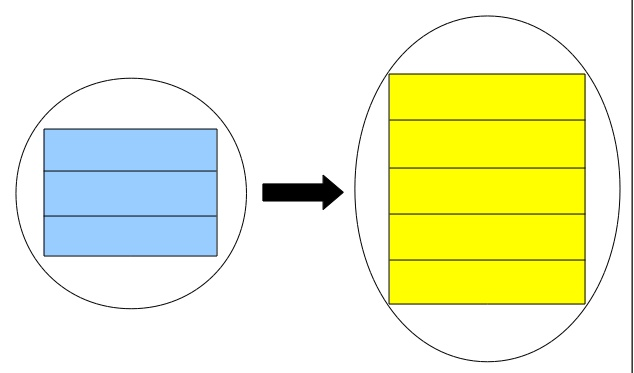
\includegraphics[scale=0.30]{figuras/vert_scaling.jpg}
    \caption{Escalabilidade Vertical}
\end{figure}
\\\\
	Uma alternativa é replicar o banco de dados em várias máquinas para permitir que o acesso seja feito de forma distribuída, evitando que um único nó torne-se um gargalo para o acesso aos dados. Ela é vantajosa quando predominam operações de leitura por parte da aplicação cliente já que, quando ocorre uma escrita no banco de dados, esta deve ser propagada para todos os nós que o compõem. Existem maneiras de amenizar este problema, porém elas esbarram na dificuldade de manter a \textbf{consistência} dos dados ao longo dos vários nós que formam o sistema. Tais abordagens que envolvem a adição de nós formando um sistema gerenciador de banco de dados distribuído são classificadas como \textbf{escalabilidade horizontal}.
\begin{figure}[h]
	\centering
	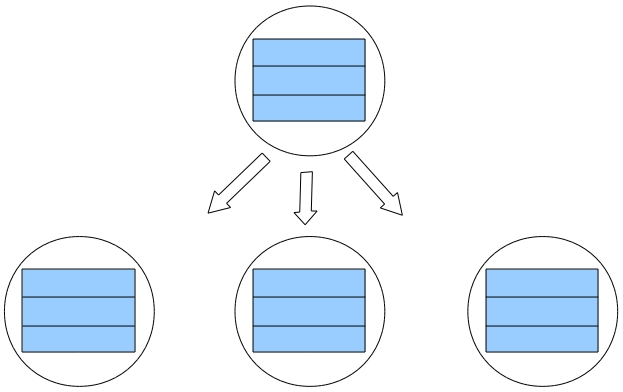
\includegraphics[scale=0.30]{figuras/horz_scaling.jpg}
    \caption{Escalabilidade Horizontall}
\end{figure}
\\\\
	A técnica de escalabilidade vertical tem como vantagem sua simplicidade: em geral nao há necessidade de reconfigurar o SGBD após sua aplicação. A escalabilidade horizontal, no entanto, apresenta um ganho de performance muito maior ao custo de um aumento de complexidade na manutenção da consistência do banco de dados, cuja responsabilidade passa a ser da aplicação cliente e não mais do SGBD.
	
\subsection{NoSQL}
	Devido à dificuldade de escalabilidade horizontal dos SGBDs relacionais, foram propostas alternativas que abrem mão de certas propriedades e garantias dadas pelo modelo relacional em troca de simplicidade e fácil escalabilidade. Os bancos de dados \textbf{NoSQL} são, em uma classificação genérica, sistemas de gerenciamento de bancos de dados que não aderem ao modelo relacional - isto é, não organizam os dados em tabelas com esquemas fixos e geralmente não usam SQL para manipulação de dados\cite{wikiNoSql}.\\\\
	Por organizarem seus dados de formas simples(abrindo mão da flexibilidade fornecida pelo modelo relacional), em geral os SGBDs NoSQL simplificam e tornam mais robusto o processo de escalabilidade horizontal\cite{IntNoSQL1}. Eles se popularizaram com a adoção desses sistemas em aplicações web de larga escala, como o \textit{Google}, \textit{Facebook} e \textit{Reddit}.
	
\subsubsection{Tipos}
	Os SGBDs NoSQL diferem nas abordagens de organização de dados. Os tipos mais comuns são:\\
	\begin{itemize}
		\item
		\textbf{Orientados a documentos}: nesses sistemas, os dados são separados em \textbf{documentos}, geralmente um por cada "linha" no equivalente relacional. A cada documento é atribuído um identificador único(uma \textit{chave}) e os atributos presentes em cada documento podem variar. Os dados podem ser acessados especificando a chave do documento procurado ou alguma propriedade do conteúdo do documento. Alguns exemplos desse tipo são \textit{Apache CouchDB}, \textit{Lotus Notes} e \textit{MongoDB}. Em particular, o serviço ilustrado nesse relatório, o \textit{Amazon SimpleDB}, faz parte dessa categoria; \\
		\item
		\textbf{Orientados a grafos}: aqui os dados são organizados segundo um modelo de \textbf{grafo}, onde cada entidade possui referências diretas a outras entidades do banco de dados. Eles são particularmente úteis para representar, por exemplo, relações de amizade em redes sociais e conectividade de estradas. São SGBDs orientados a grafos o \textit{Neo4J}, o \textit{InfiniteGraph} e \textit{FlockDB}; \\
		\item
		\textbf{Bancos chave-valor}: os bancos de dados chave-valor permitem que os dados sejam armazenados sem o uso de um esquema fixo. Cada entrada de dados consiste em uma \textit{string} que representa a \textbf{chave} e os dados correspondentes, que formam o \textbf{valor} associado à chave. SGBDs NoSQL como \textit{Apache Cassandra}, \textit{Redis} e \textit{Amazon DynamoDB} seguem essa abordagem.\\
	\end{itemize}
